\documentclass{handout}

\SetInstructor{Lt Col James Phillips}
\SetCourseTitle{ECE231: Electrical Circuits and Systems I}
\SetSemester{Spring 2016}
\SetHandoutTitle{Lecture 8: Linearity and Superposition}
%\SetDueDate{1 Jan 2016}
%\ShowAllBlanks

\showsoln \setsolncolor{red}

\begin{document}
\maketitle

\textbf{Upcoming events}
\begin{enumerate}
\item HW \#3 due Lesson 10
\item Problem set \#2 due Lesson 10
\item Quiz \#2 during Lesson 10
\item GR \#1 Lesson 12
\end{enumerate}

\textbf{OBJECTIVES:}
\begin{enumerate}
\item Understand what is meant by a {\em Linear} Circuit
\item Understand and be able to apply the principle of superposition
\end{enumerate}

\textbf{READING}
\begin{description}
\item [Required]:
\begin{itemize}
\item  Textbook, sections 3.3, pages 100--109
\end{itemize}
\item [Optional]: None
\end{description}

\textbf{HOMEWORK}
\begin{description}
\item [Required textbook problems]: 3.36, 3.38--- Due Lesson 10
\item [Recommended textbook problems]: 3.39
\end{description}


\section{What does it mean for a circuit to be Linear?}
Circuits are linear when they can be modeled using only linear elements and independent sources.  Further any linear circuit will obey the following 2 principles:
\begin{description}
\item[Homogeneity]-- outputs are proportional to the inputs. This is also referred to as \textbf{proportionality}.
\item[Additivity]: output due to multiple inputs can be found by finding the output due to each individual input and then adding them.  This is also referred to as \textbf{superposition}; we will devote an entire section to this later.
\end{description}

Mathematically these properties are written as:
\soln{3}{
\begin{equation}
f(Kx) = Kf(x)
\end{equation}
\begin{equation}
f(x_1+x_2)=f(x_1)+f(x_2)
\end{equation}
}

\newpage
\clearpage
\pagebreak

\textbf{Example 1:} Solve for $v_{out}$ in the circuit in Figure \ref{fig: Example1} given $v_{in} = 1V$.  Then using the proportionality principle, find the output given  $v_{in}=12V$
\begin{figure} [h t b]
\centering
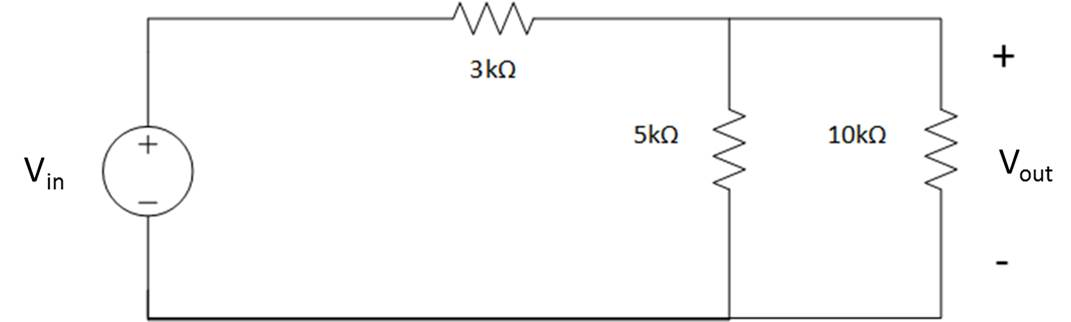
\includegraphics[width=0.7\textwidth]{Example1.jpg}
\caption{Circuit to accompany example 1}
\label{fig: Example1}
\end{figure}

\soln{6in}{
\begin{figure} [h t b]
\centering
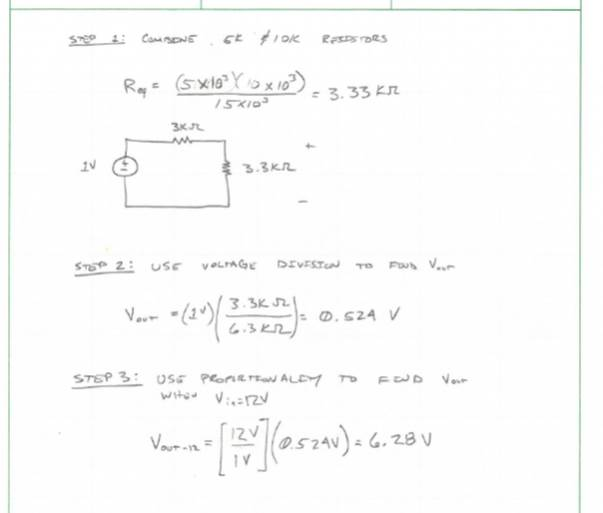
\includegraphics[width=0.8\textwidth]{Example1soln.jpg}
\end{figure}
}

\newpage
\clearpage
\pagebreak

\section{Superposition (Additivity)}
The goal of superposition is to simplify the analysis of circuits with multiple sources by only having to deal with a single source at a time.  Notice, I said it is simpler not shorter.

\soln{4in}{
The steps for circuit analysis using superposition are:
\begin{enumerate}
\item {\em Turn off} all but one of the independent sources in the circuit
\item Solve for output of the circuit based on the one remaining source
\item Repeat for every source in the circuit
\item Sum the results to get a total output
\end{enumerate}
}

\textbf{What do we mean by turning off sources?}
\begin{description}
\item[To turn off a voltage source,] we would want the voltage across the two nodes of the source to be zero, so we replace the source with a short circuit
\item[To turn off a current source,] we want zero current to flow, so we replace it with an open circuit
\end{description}

\textbf{Example 2:} Without solving anything else, re-draw the circuit in Figure \ref{fig: Example2} with each source turned off.
\begin{figure} [h t b]
\centering
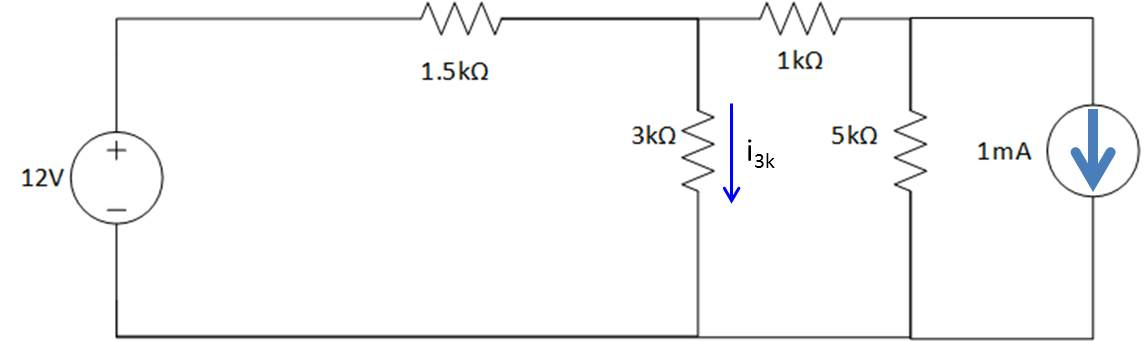
\includegraphics[width=0.7\textwidth]{Example2.jpg}
\caption{Circuit to accompany example 2}
\label{fig: Example2}
\end{figure}

\soln{6in}{
\begin{figure} [h t b]
\centering
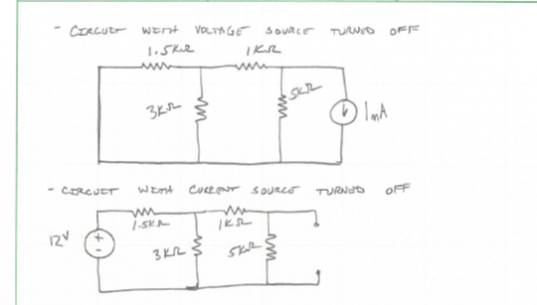
\includegraphics[width=0.8\textwidth]{Example2soln.jpg}
\end{figure}
}

\newpage
\clearpage
\pagebreak

\textbf{Example 3:} (Textbook Exercise 3-25) -- The circuit in Figure \ref{fig: Example3} contains two $R$--$2R$ modules.  Use superposition to find $v_O$.  NOTE: In images taken from the textbook, crossed wires are only connected if they are {\em dotted}.  For circuits that I draw on the board or ones I generate for notes, crossed wires are connections.  You will need to learn to infer from context...... If there are some {\em dotted} nodes, crossed wires without dots are not connected; if there are no dots, crossed wires are connected.
\begin{figure} [h t b]
\centering
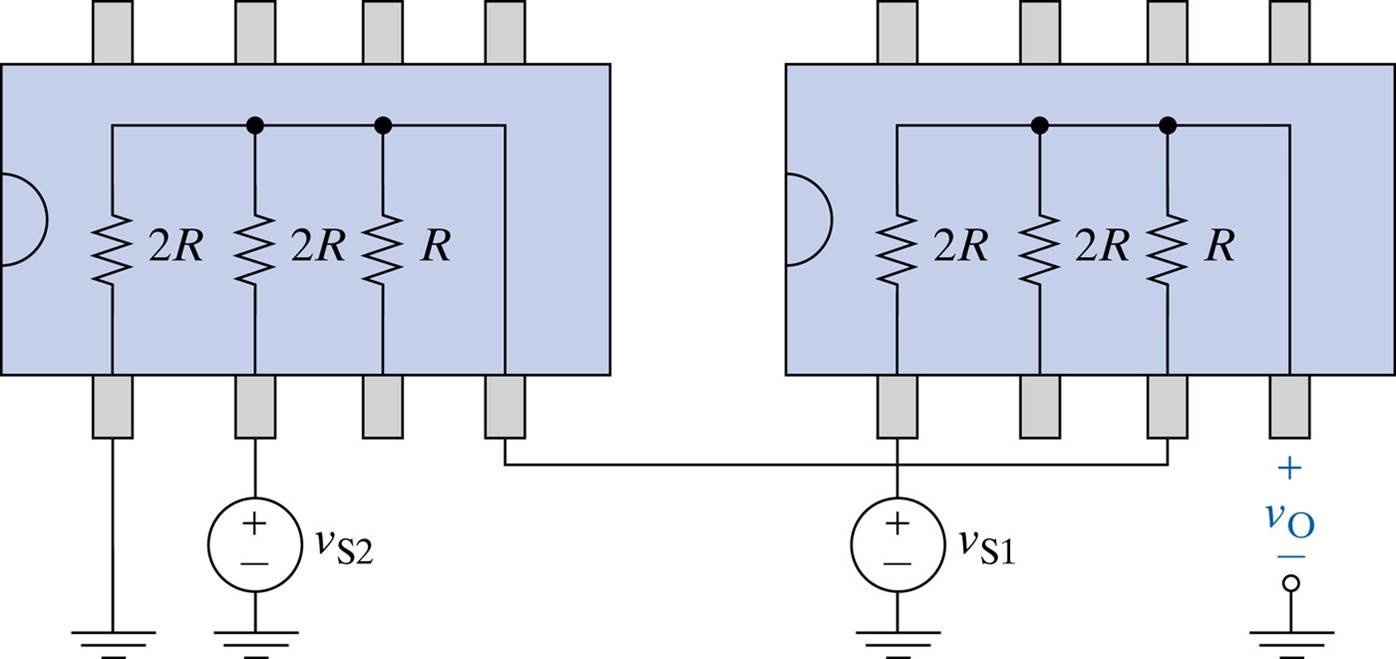
\includegraphics[width=0.7\textwidth]{Example3.jpg}
\caption{Circuit to accompany example 3}
\label{fig: Example3}
\end{figure}

\soln{6in}{
\begin{figure} [h t b]
\centering
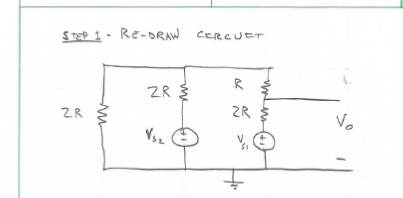
\includegraphics[width=0.8\textwidth]{Example3solnA.jpg}
\end{figure}

\begin{figure} [h t b]
\centering
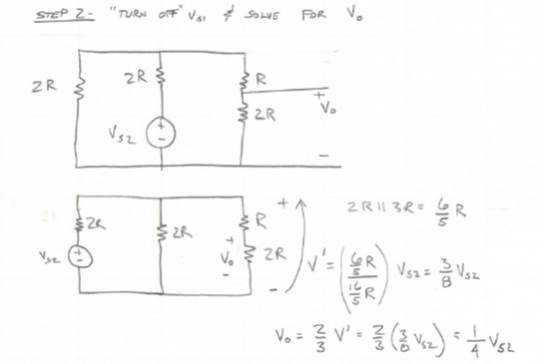
\includegraphics[width=0.7\textwidth]{Example3solnB.jpg}
\end{figure}

\begin{figure} [h t b]
\centering
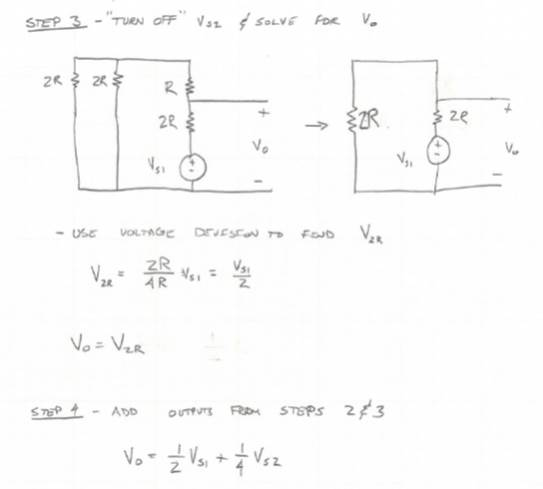
\includegraphics[width=0.7\textwidth]{Example3solnC.jpg}
\end{figure}
}

\newpage
\clearpage
\pagebreak

\textbf{Example 4:} (Textbook Exercise 3-26) -- Repeat the above example, but replace $v_{s2}$ in Figure \ref{fig: Example3} with a current source, $i_{s2}$ with the reference arrow pointed toward ground

\soln{6in}{
\begin{figure} [h t b]
\centering
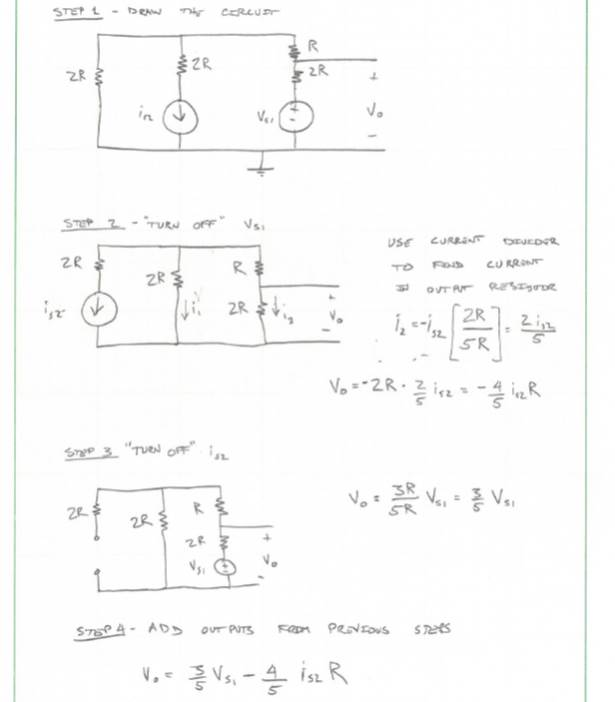
\includegraphics[width=0.9\textwidth]{Example4soln.jpg}
\end{figure}

}

\newpage
\clearpage
\pagebreak

\textbf{Example 5:}  Use Superposition to find $v_O$ in Figure \ref{fig: Example5}
\begin{figure} [h t b]
\centering
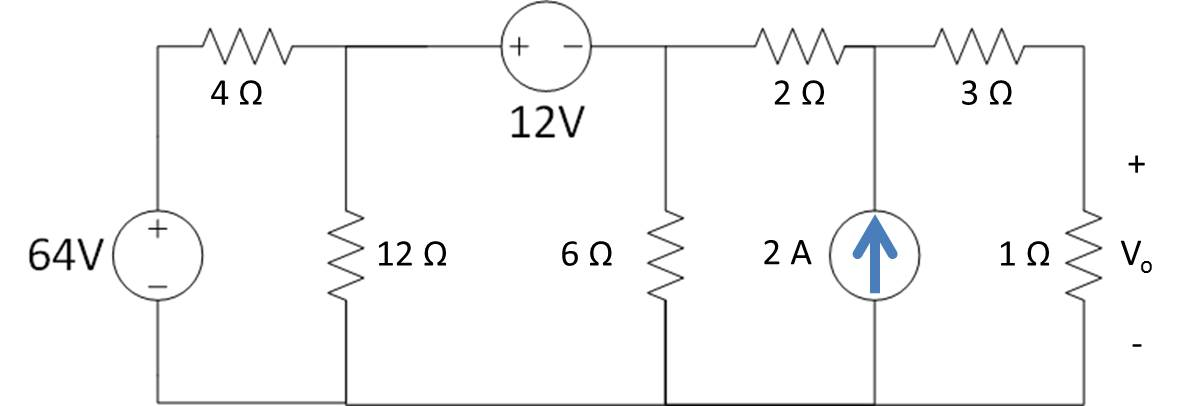
\includegraphics[width=0.6\textwidth]{Example5.jpg}
\caption{Circuit to accompany example 5}
\label{fig: Example5}
\end{figure}

\soln{6in}{
\begin{figure} [h t b]
\centering
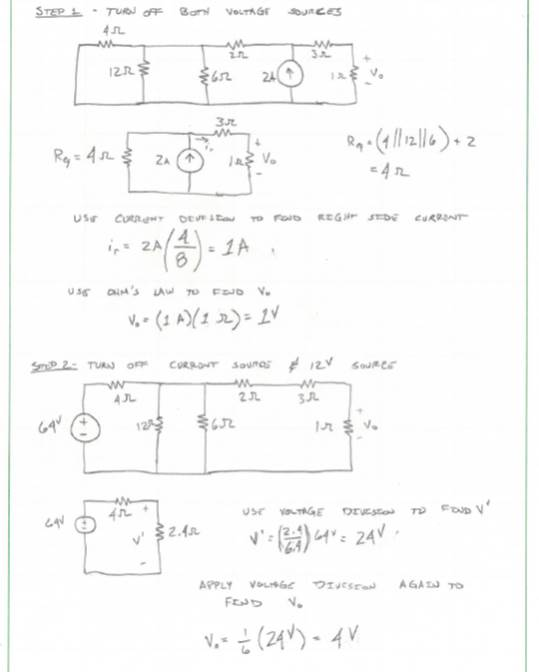
\includegraphics[width=0.6\textwidth]{Example5solnA.jpg}
\end{figure}

\begin{figure} [h t b]
\centering
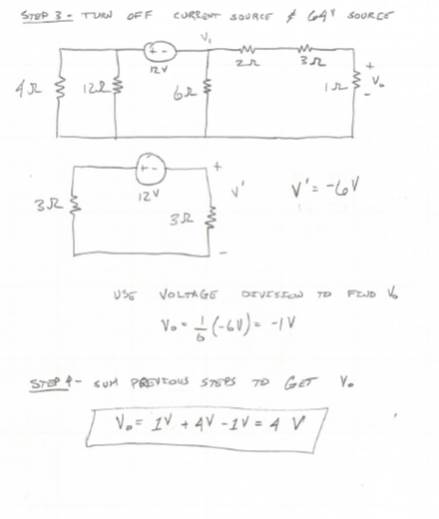
\includegraphics[width=0.9\textwidth]{Example5solnB.jpg}
\end{figure}

}



\newpage
\clearpage
\pagebreak




\end{document}


% Equation Array Example Code
%\begin
%{eqnarray}
%P_R &=& i_R^2R \nonumber \\
%P_R &=& (100\ mA)^2 \times 100\ \Omega \nonumber \\
%P_R &=& (100 \times 10^{-3}\ A)^2 \times 100\ \Omega \\
%P_R &=& 10000 \times 10^{-6}\ A^2  \times 100\ \Omega \nonumber \\
%P_R &=& 1\ W  \nonumber
%\end{eqnarray} 

% Figure Example Code
%\begin{figure} [h t b]
%\centering
%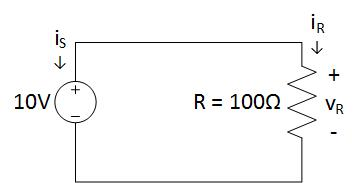
\includegraphics[width=0.5\textwidth]{OhmsLawExampleSolution.jpg}
%\caption{Ohm's Law example circuit}
%\label{fig: OhmsLawExampleSolution}
%\end{figure}

%Table Example Code
%\begin{table}[h]
%\centering
%\begin{tabular}{|l|c|c|}
%\hline
%Prefix & Abbreviation & Value \\
%\hline \hline
%Giga & $G$ & $10^9$ \\
%Mega & $M$ & $10^6$ \\
%Kilo & $k$ & $10^3$ \\
%\hline
%milli & $m$ & $10^{-3}$ \\
%micro & $\mu$ & $10^{-6}$ \\
%nano & $n$ & $10^{-9}$ \\
%pico & $p$ & $10^{-12}$ \\
%\hline
%\end{tabular}
%\caption{Engineering prefixes and values}
%\label{tab: Eng Prefixes}
%\end{table}
